\chapter{Supplemental figures}
\begin{figure}[thbp]
\centering
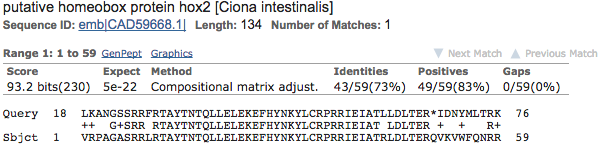
\includegraphics[scale=0.75]{figures/occi_hox2.png}
\caption{\textbf{Alignment of \textit{M. occidentalis} \textit{hox2} genes alignment with \textit{Ciona} show  premature stop codon.} Two copies of \textit{hox10} were found in \textit{M. occidentalis} \mytilde12 kb apart on the same contig.}
\label{fig:occihox2}
\end{figure}

\begin{figure}[tbp]
\centering
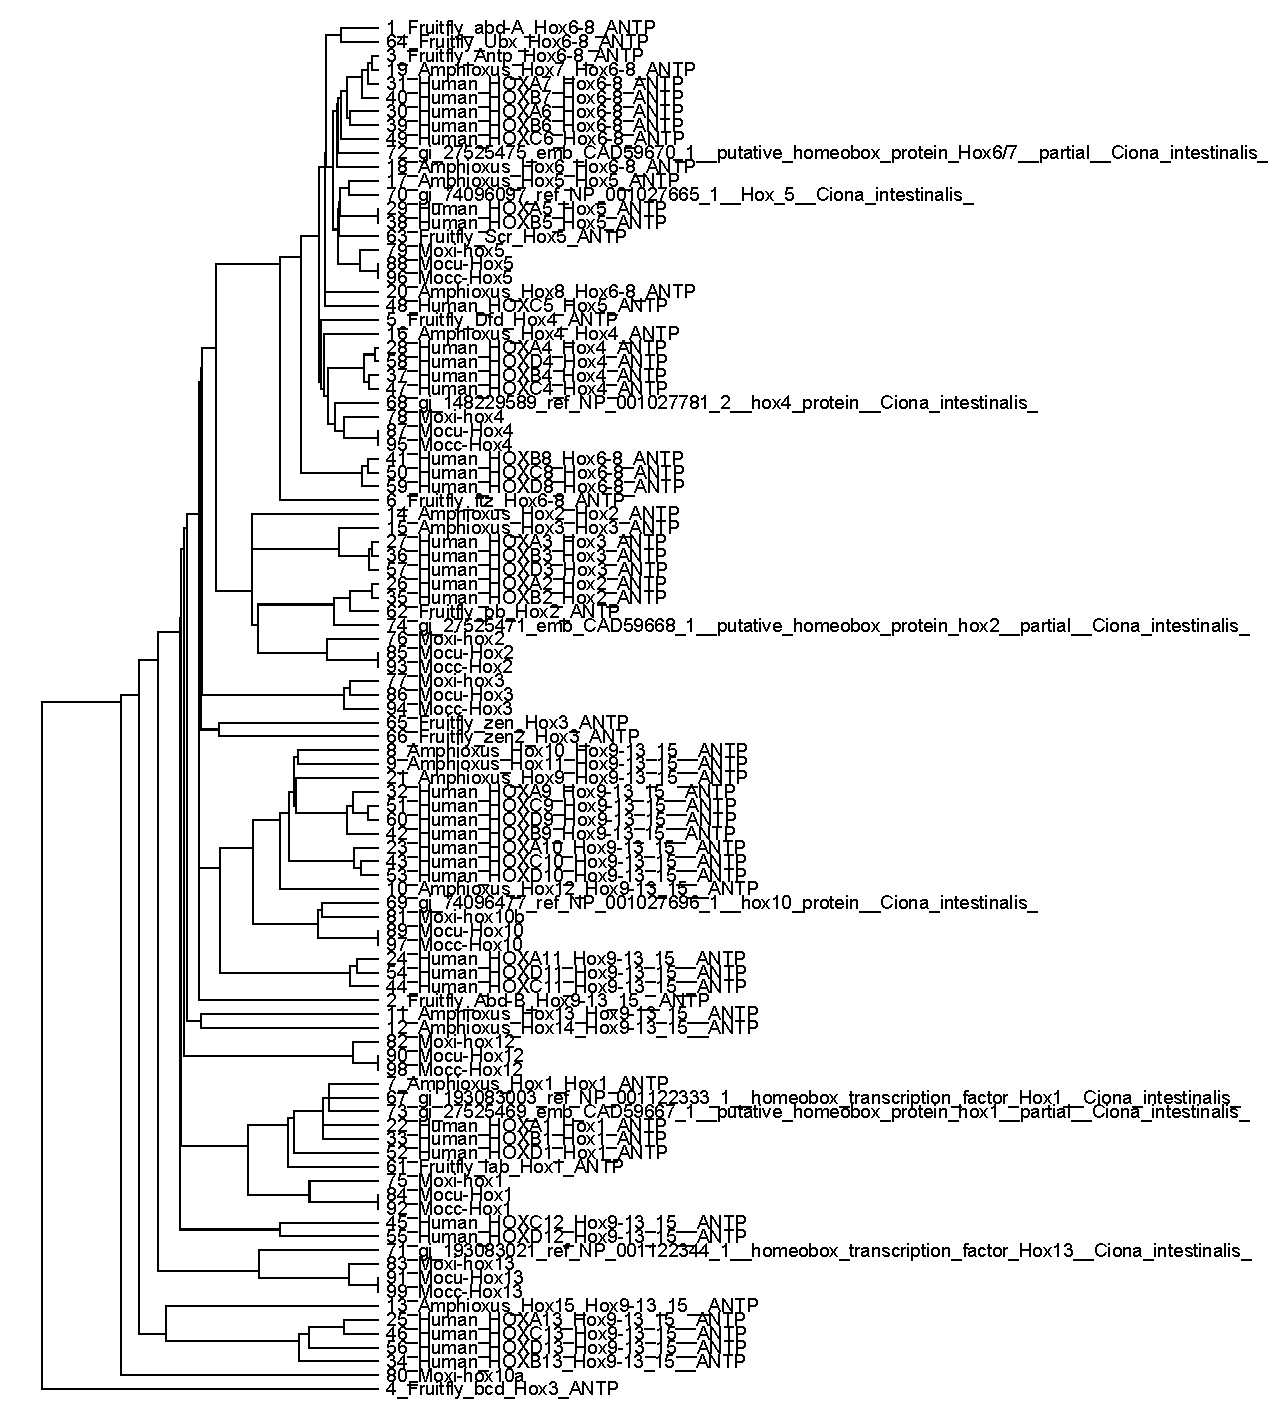
\includegraphics[scale=0.85]{figures/hox_alignment.pdf}
\caption{\textbf{Alignment of \textit{hox} genes.} Two copies of \textit{hox10} were found in \textit{M. occidentalis} \mytilde12 kb apart on the same contig.}
\label{fig:hox-alignments}
\end{figure}

\begin{figure}[tbp]
\centering
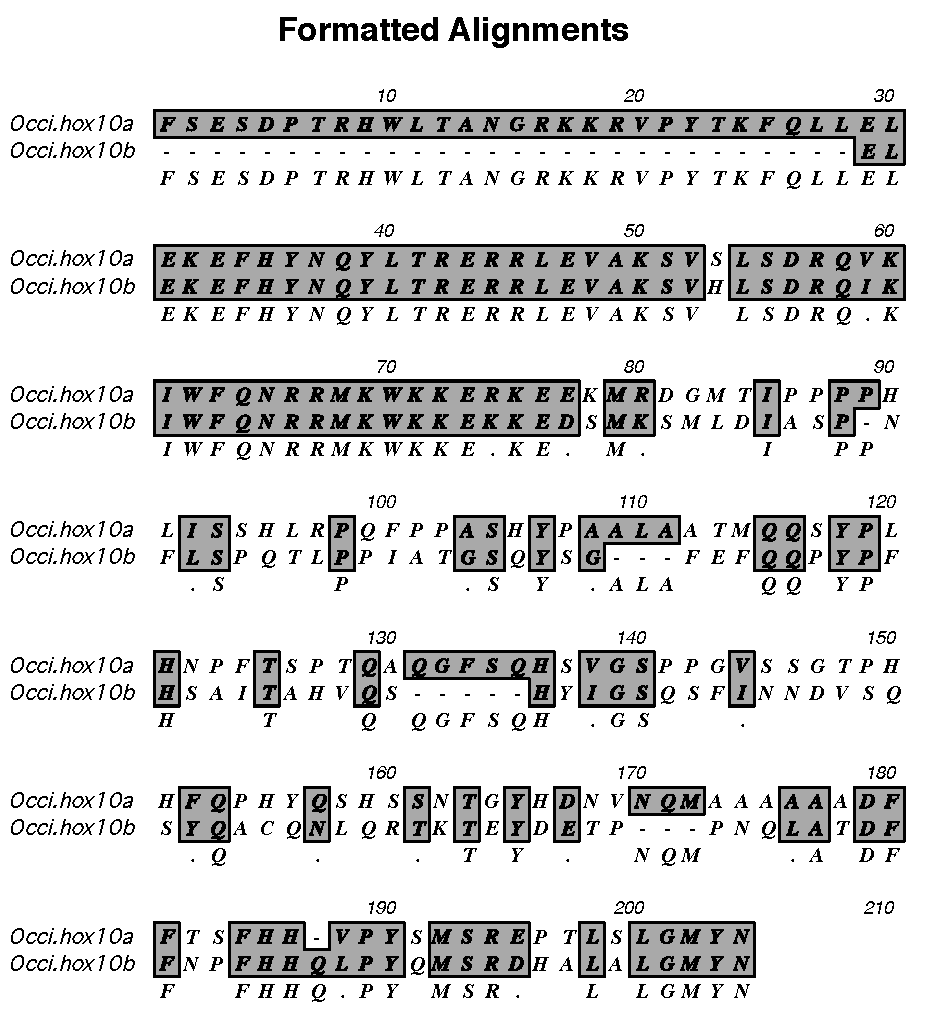
\includegraphics[scale=0.95]{figures/Occi_hox10.pdf}
\caption{\textbf{Alignment of \textit{M. occidentalis} duplicate \textit{hox10} genes} Two copies of \textit{hox10} were found in \textit{M. occidentalis} \mytilde12 kb apart on the same contig.}
\label{fig:occihox10}
\end{figure}